\section{梯度下降解多元线性回归}
\label{sec:chapter2}

\subsection{多元线性回归}

类似于一元的线性回归，不过我们现在有多个自变量 $x_1,x_2,\cdots,x_n$，即给定的数据集为：
\[
\left\{\left(x_1^{(i)},x_2^{(i)},\cdots,x_n^{(i)},y^{(i)}\right),\;i=1,2,\cdots,m\right\}
\]
相应地，回归方程也具有多个参数 $\theta_0,\theta_1,\cdots,\theta_n$：
\[
h_\theta(x)=\theta^Tx=\theta_0x_0+\cdots+\theta_nx_n
\]
这里我们假定 $x_0$ 恒等于 $1$，并以向量表示自变量和参数：$\theta=(\theta_0,\cdots,\theta_n)^T,\;x=(x_0,\cdots,x_n)^T$. 



\subsection{梯度下降解多元线性回归}

类似的，我们定义代价函数：
\[
J(\theta)=\frac{1}{2m}\sum_{i=1}^m\left(\theta^Tx^{(i)}-y^{(i)}\right)^2
\]
于是，
\[
\frac{\partial J}{\partial \theta}=\frac{1}{m}\sum_{i=1}^m\left(\theta^Tx^{(i)}-y^{(i)}\right)x^{(i)}
\]
梯度下降时，不断作迭代：
\[
\theta:=\theta-\alpha\cdot\frac{\partial J}{\partial \theta}
\]
即可。


\paragraph{特征缩放与标准化}

当我们的不同自变量取值范围相差较大时，梯度下降可能会很慢，这时，我们需要把所有自变量进行缩放、标准化。具体的，只要我们置：
\[
x_i^{(j)}:=\frac{x_i^{(j)}-\mu_i}{\sigma_i}
\]
其中，$\mu_i=\frac{1}{m}\sum\limits_{j=1}^m x_i^{(j)}$ 是样本均值，$\sigma_i=\sqrt{\frac{\sum\limits_{j=1}^m\left(x_i^{(j)}-\mu_i\right)^2}{m-1}}$ 是样本标准差，就完成了归一化。

归一化后样本均值为 $0$，方差为 $1$. 


\paragraph{代码实现}

\texttt{Normalization} 函数将数据集标准化，\texttt{J} 函数即计算 $J(\theta)$，\texttt{partJ} 函数计算 $\frac{\partial J}{\partial\theta}$，\texttt{GradientDescent} 进行梯度下降。

\begin{lstlisting}[language=Python]
import numpy as np
import matplotlib.pyplot as plt

alpha = 0.01
iteration = 10000
Z = []

def Normalization(data):
	return (data - data.mean(axis = 0)) / data.std(axis = 0, ddof = 1)

def J(T, X, Y):
	res = 0
	for i in range(m):
		res += (np.matmul(T.T, X[i:i+1, :].T) - Y[i:i+1, :]) ** 2
	res /= 2 * m;
	return res

def partJ(T, X, Y):
	res = np.zeros((n, 1))
	for i in range(m):
		res += (np.matmul(T.T, X[i:i+1, :].T) - Y[i:i+1, :]) * X[i:i+1, :].T
	res /= m
	return res

def GradientDescent(X, Y):
	T = np.zeros((n, 1))
	for t in range(iteration):
		T = T - alpha * partJ(T, X, Y)
		Z.append(J(T, X, Y)[0][0])
	return T

data = np.genfromtxt("ex1data2.txt", delimiter = ',')
(m, n) = data.shape
data = Normalization(data)
X = np.column_stack((np.ones((m, 1)), data[:, :-1]))
Y = data[:, -1:]
T = GradientDescent(X, Y)
print(T)

p1 = plt.subplot(111)
p1.plot(range(1, iteration+1), Z)
p1.set_xlabel('Iteration')
p1.set_ylabel('Cost')
plt.show()
\end{lstlisting}

最后得到的结果：$\theta=(-1.11051830\times10^{-16},8.84765988\times10^{-1},-5.31788197\times10^{-2})^T$. 

学习率取为 $0.01$ 时，代价函数值随迭代次数的变化：

\begin{figure}[H]
    \centering
    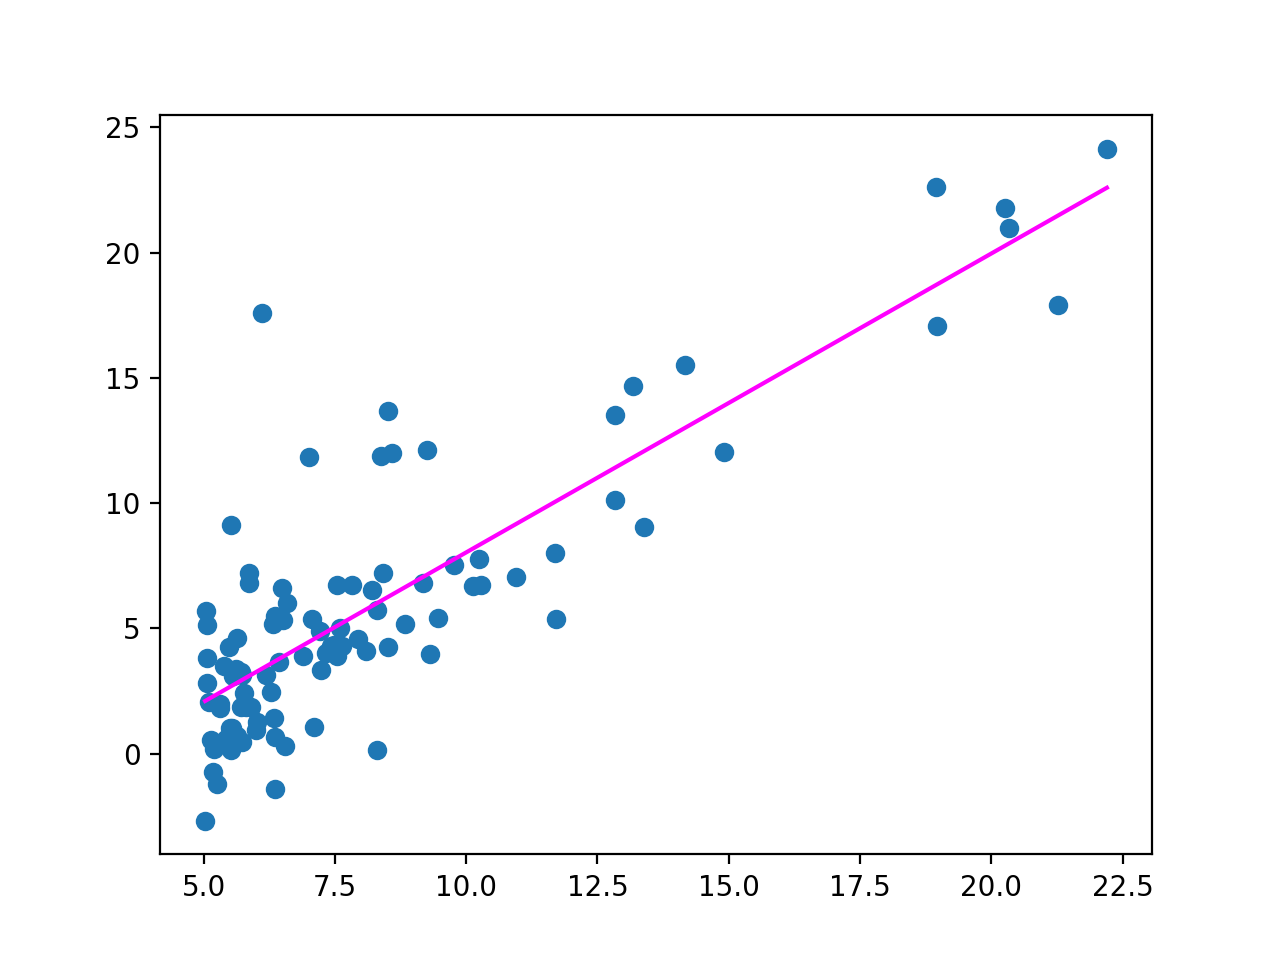
\includegraphics[width=0.5\linewidth]{figs/Chap_1_Figure_2.png}
\end{figure}